% Copyright 2005-2016 Airbus-EDF-IMACS-Phimeca
% Permission is granted to copy, distribute and/or modify this document
% under the terms of the GNU Free Documentation License, Version 1.2
% or any later version published by the Free Software Foundation;
% with no Invariant Sections, no Front-Cover Texts, and no Back-Cover
% Texts.  A copy of the license is included in the section entitled "GNU
% Free Documentation License".
\renewcommand{\filename}{docUC_StochProc_RandomWalk.tex}
\renewcommand{\filetitle}{UC : Creation of a Random Walk}

% \HeaderNNIILevel
% \HeaderIILevel
\HeaderIIILevel

\label{processWN}

\index{Stochastic Process!Random Walk}


This section details first how to create and manipulate a random walk.\\

A random walk $X: \Omega \times \cD \rightarrow \Rset^d$ is a  process where $\cD=\Rset$ discretized on the time grid $(t_i)_{i \geq 0}$ such that:
\begin{eqnarray}
  X_{t_0} & = & \vect{x}_{t_0} \\
  \forall n>0,\: X_{t_n} & = & X_{t_{n-1}} + \varepsilon_{t_n}
\end{eqnarray}
where $\vect{x}_0 \in \Rset^d$ and $\varepsilon$ is a  white noise of dimension $d$.\\

OpenTURNS proposes to model it through the object \emph{RandomWalk} defined thanks to the origin, the distribution of the white noise and the time grid.\\


\requirements{
  \begin{description}
  \item[$\bullet$] a numerical point : {\itshape \textit{myOrigin}}
  \item[type:] NumericalPoint
  \end{description}

  \begin{description}
  \item[$\bullet$] two distributionq : {\itshape \textit{myDist}}
  \item[type:]  Distribution
  \end{description}

  \begin{description}
  \item[$\bullet$] a time grid : {\itshape \textit{myTimeGrid}}
  \item[type:]  RegularGrid
  \end{description}

}
{
  \begin{description}
  \item[$\bullet$] a random walk {\itshape myRandomWalk}
  \item[type:]  RandomWalk
  \end{description}
}

\textspace\\
Python script for this UseCase :

\inputscript{script_docUC_StocProc_RandomWalk}

\textspace\\
Figures (\ref{randomwalk1D_Discrete}) and (\ref{randomwalk1D_Continuous}) illustrate realizations of a 1D random walk where the distribution $\cD$ is respectively :
\begin{itemize}
\item discrete :  the support is the two points $\{-1, 10\}$ with respective weights $0.9$ and $0.1$,
\item continuous : the Normal distribution $\cN(0,1)$.
\end{itemize}



\begin{figure}[H]
  \begin{minipage}{9cm}
    \begin{center}
      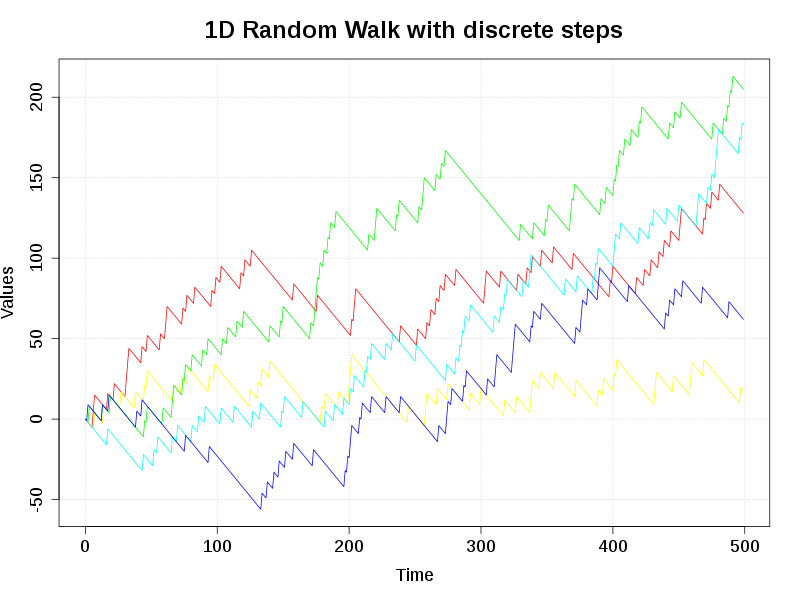
\includegraphics[width=7cm]{Figures/randomwalk1D_discrete.png}
      \caption{Realizations of a random walk with the discrete distribution : $P(-1) = 0.9, P(10)=0.1$.}
      \label{randomwalk1D_Discrete}
    \end{center}
  \end{minipage}
  \hfill
  \begin{minipage}{9cm}
    \begin{center}
      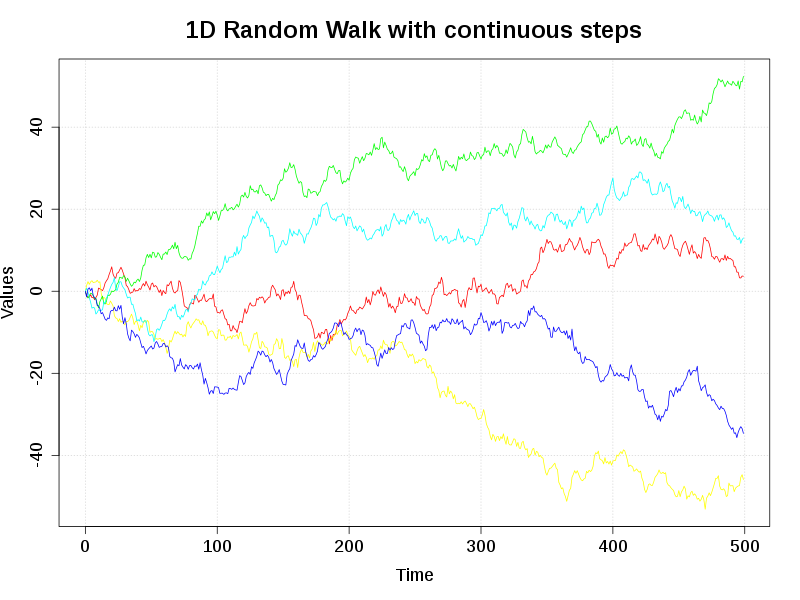
\includegraphics[width=7cm]{Figures/randomwalk1D_continuous.png}
      \caption{Realizations of a random walk with distribution $\cN(0,1)$.}
      \label{randomwalk1D_Continuous}
    \end{center}
  \end{minipage}
\end{figure}

Figures (\ref{randomwalk2D_Discrete}) and (\ref{randomwalk2D_Continuous}) illustrate realizations of a 2D random walk where the distribution $\cD$ is respectively :
\begin{itemize}
\item discrete :  the support is the two points $\{-1, 10\}$ with respective weights $0.9$ and $0.1$,
\item continuous : the 2D Normal distribution $\cN(\vect{0},\mat{1})$.
\end{itemize}
The realizations are  presented in the phase space $X_1$ versus $X_2$.


\begin{figure}[H]
  \begin{minipage}{9cm}
    \begin{center}
      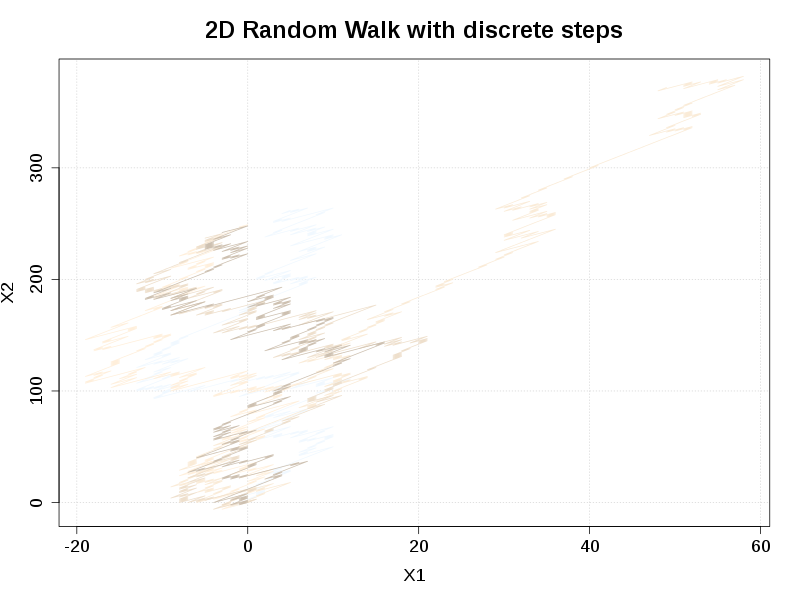
\includegraphics[width=7cm]{Figures/randomwalk2D_discrete.png}
      \caption{Realizations of a random walk with the uniform discrete distribution over the points $(-1, -2)$ and $(1,3)$.}
      \label{randomwalk2D_Discrete}
    \end{center}
  \end{minipage}
  \hfill
  \begin{minipage}{9cm}
    \begin{center}
      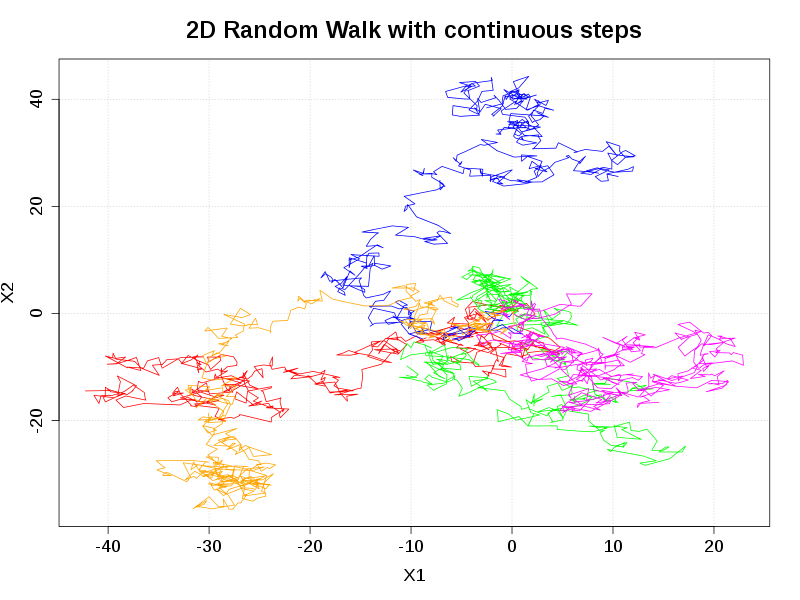
\includegraphics[width=7cm]{Figures/randomwalk2D_continuous.png}
      \caption{5 realizations of a random walk with distribution $\cN(\vect{0},\mat{I})$}
      \label{randomwalk2D_Continuous}
    \end{center}
  \end{minipage}
\end{figure}
